\section{改进的 {\kvcache} 缓存系统}
\label{sec:design}

\subsection{设计空间概览}
\label{sec:design-mechanism}

现有 {\kvcache} 缓存系统~\cite{cachedattention,vllm,sglang,DBLP:journals/corr/abs-2403-14401} 采用相似的缓存机制与策略。下面先简要概述这些设计，再介绍本文改进的策略。

\stitle{当前 {\kvcache} 缓存机制与策略。}
在机制方面，现有系统主要以分层方式在 GPU 和 CPU 上缓存 {\kvcache}。{\kvcache} 以块为粒度管理（见第~\ref{sec:bg} 节）：产生一个 {\kvcache} 块时，首先将其缓存在 GPU HBM；如果 GPU 因内存不足而无法缓存新生成的块，缓存系统会采用下述淘汰策略，从 GPU 向 CPU 淘汰一些块。被淘汰块按层异步换出到 CPU，因而换出开销可忽略。如果 CPU 也耗尽内存，则删除这些块。执行新请求前，若请求命中缓存块，服务系统会直接复用，避免重复计算。若命中位于 CPU，块也会按层换入 GPU。

在策略方面，{\kvcache} 缓存系统主要需要两种策略：如何判断缓存命中，以及如何淘汰缓存块。对前者，不同设计检查潜在命中块的粒度不同：一些系统跨所有请求检查匹配~\cite{sglang,DBLP:journals/corr/abs-2404-12457}，另一些仅在单个用户的请求内部检查匹配~\cite{DBLP:journals/corr/abs-2403-14401,cachedattention}。对后者，当前系统主要采用 LRU 或 FIFO 等标准淘汰策略。尽管它们会加入一些扩展，例如检查待淘汰块是否仍在调度队列~\cite{cachedattention}，总体原理并未改变。

\stitle{缺点。}
LRU 等现有工作负载无关策略可能忽略第~\ref{sec:analyze} 节分析的工作负载特征，因而并非最优。以轨迹 A 为例，在距上次访问经过相同时间（例如超过 10 秒）的情况下，10 轮 Text 请求比 1 轮 Text 请求更可能继续发起下一轮（见\fig{fig:motiv-next-turn-probability}）。然而，如果大量 1 轮请求涌入系统，由于 10 轮请求的复用时间更长，它们仍可能被 LRU 淘汰。

\begin{table}[!t]
    \centering
    \small
    \resizebox{\linewidth}{!}{
        \ra{1.2}
        \begin{tabular}{@{}p{0.45\linewidth}p{0.45\linewidth}@{}}
            \toprule
            \textbf{观察} & \textbf{技术} \\ \midrule
            给定工作负载后，{\kvcache} 复用概率服从指数分布（\fig{fig:motiv-next-turn-probability}与\fig{fig:motiv-reuse-time-probability-hist}）。
            & \ding{192} 基于工作负载感知复用概率分布的优先级估计。 \\
            空间局部性（\fig{fig:motiv-spatial}--\ref{fig:motiv-spatial-workload}）。
            & \ding{193} 为前部 {\kvcache} 块赋予更高优先级。 \\
            {\kvcache} 生命周期短暂（\fig{fig:motiv-block-timespan}）。
            & \ding{194} 计算优先级时移除频率，并限制概率计算的时间跨度。 \\
            \bottomrule
        \end{tabular}
    }
    \caption{依据第~\ref{sec:analyze} 节中的发现，对工作负载感知缓存淘汰策略主要技术的总结。}
    \label{tab:insights}
\end{table}


\stitle{本文方案：基于工作负载感知复用概率分布的 {\kvcache} 淘汰策略。}
为此，我们依据第~\ref{sec:motiv-temporal-spatial} 节中的特征刻画，提出一种考虑各请求类别复用概率分布的工作负载感知缓存淘汰策略。总体而言，发生淘汰时，本文会为每个块计算一个优先级，即依据其请求类别（工作负载）经分析得到的复用概率分布，估计该 {\kvcache} 未来被复用的可能性。该优先级还综合考虑空间局部性以及 {\kvcache} 块的短暂生命周期，优先淘汰优先级最低的块。表~\ref{tab:insights}总结了本文技术及其在第~\ref{sec:analyze} 节中对应的观察。

本文的缓存机制沿用现有系统~\cite{cachedattention,vllm,sglang,DBLP:journals/corr/abs-2403-14401}，包括异步换出与流水化加载，因为这些技术已经收敛为标准设计。

\subsection{工作负载感知的 {\kvcache} 缓存淘汰策略}
\label{sec:design-policy}

\nospacestitle{现有工作负载感知策略。}
工作负载感知的缓存淘汰策略已得到广泛研究~\cite{cherkasova1998improving,lruk,slru,lirs,arc,lhd,cacheus}。一个代表性策略是 Greedy-Dual-Frequency-Size（GDFS）~\cite{cherkasova1998improving}，它使用下列与工作负载相关的特征来评估每个缓存对象（例如 {\kvcache}）的优先级：
\[
\text{Priority}=\text{Clock}+\frac{\text{Frequency}\times\text{Cost}}{\text{Size}}\quad(\text{现有 GDFS}) .
\]
其中，\texttt{Clock} 捕获对象上次访问时间（与 LRU 类似），\texttt{Frequency} 是对象累计访问次数（与 LFU 类似），\texttt{Size} 是缓存对象大小，\texttt{Cost} 是把缓存内容重新带回缓存的代价。优先级最低的对象最先被淘汰。

尽管可调整上述 GDFS 公式来计算 {\kvcache} 块的优先级，但我们发现，它并未充分考虑 LLM 服务中的 {\kvcache} 使用情况，以及不同请求类别已知的概率分布。例如，由于 {\kvcache} 块生命周期很短，一个被频繁访问的块未来也可能不再复用，使一个“曾频繁访问但已经死亡”的块浪费 {\kvcache} 空间。此外，把某个块带回缓存的代价更高，并不意味着其未来更可能被复用；应当优先把更可能复用的块带回缓存。在 GDFS 的设置中无法获得这类工作负载信息，但依据上一节的特征刻画，LLM 服务系统可以直接获得它们。

\begin{figure}[!t]
    \centering
    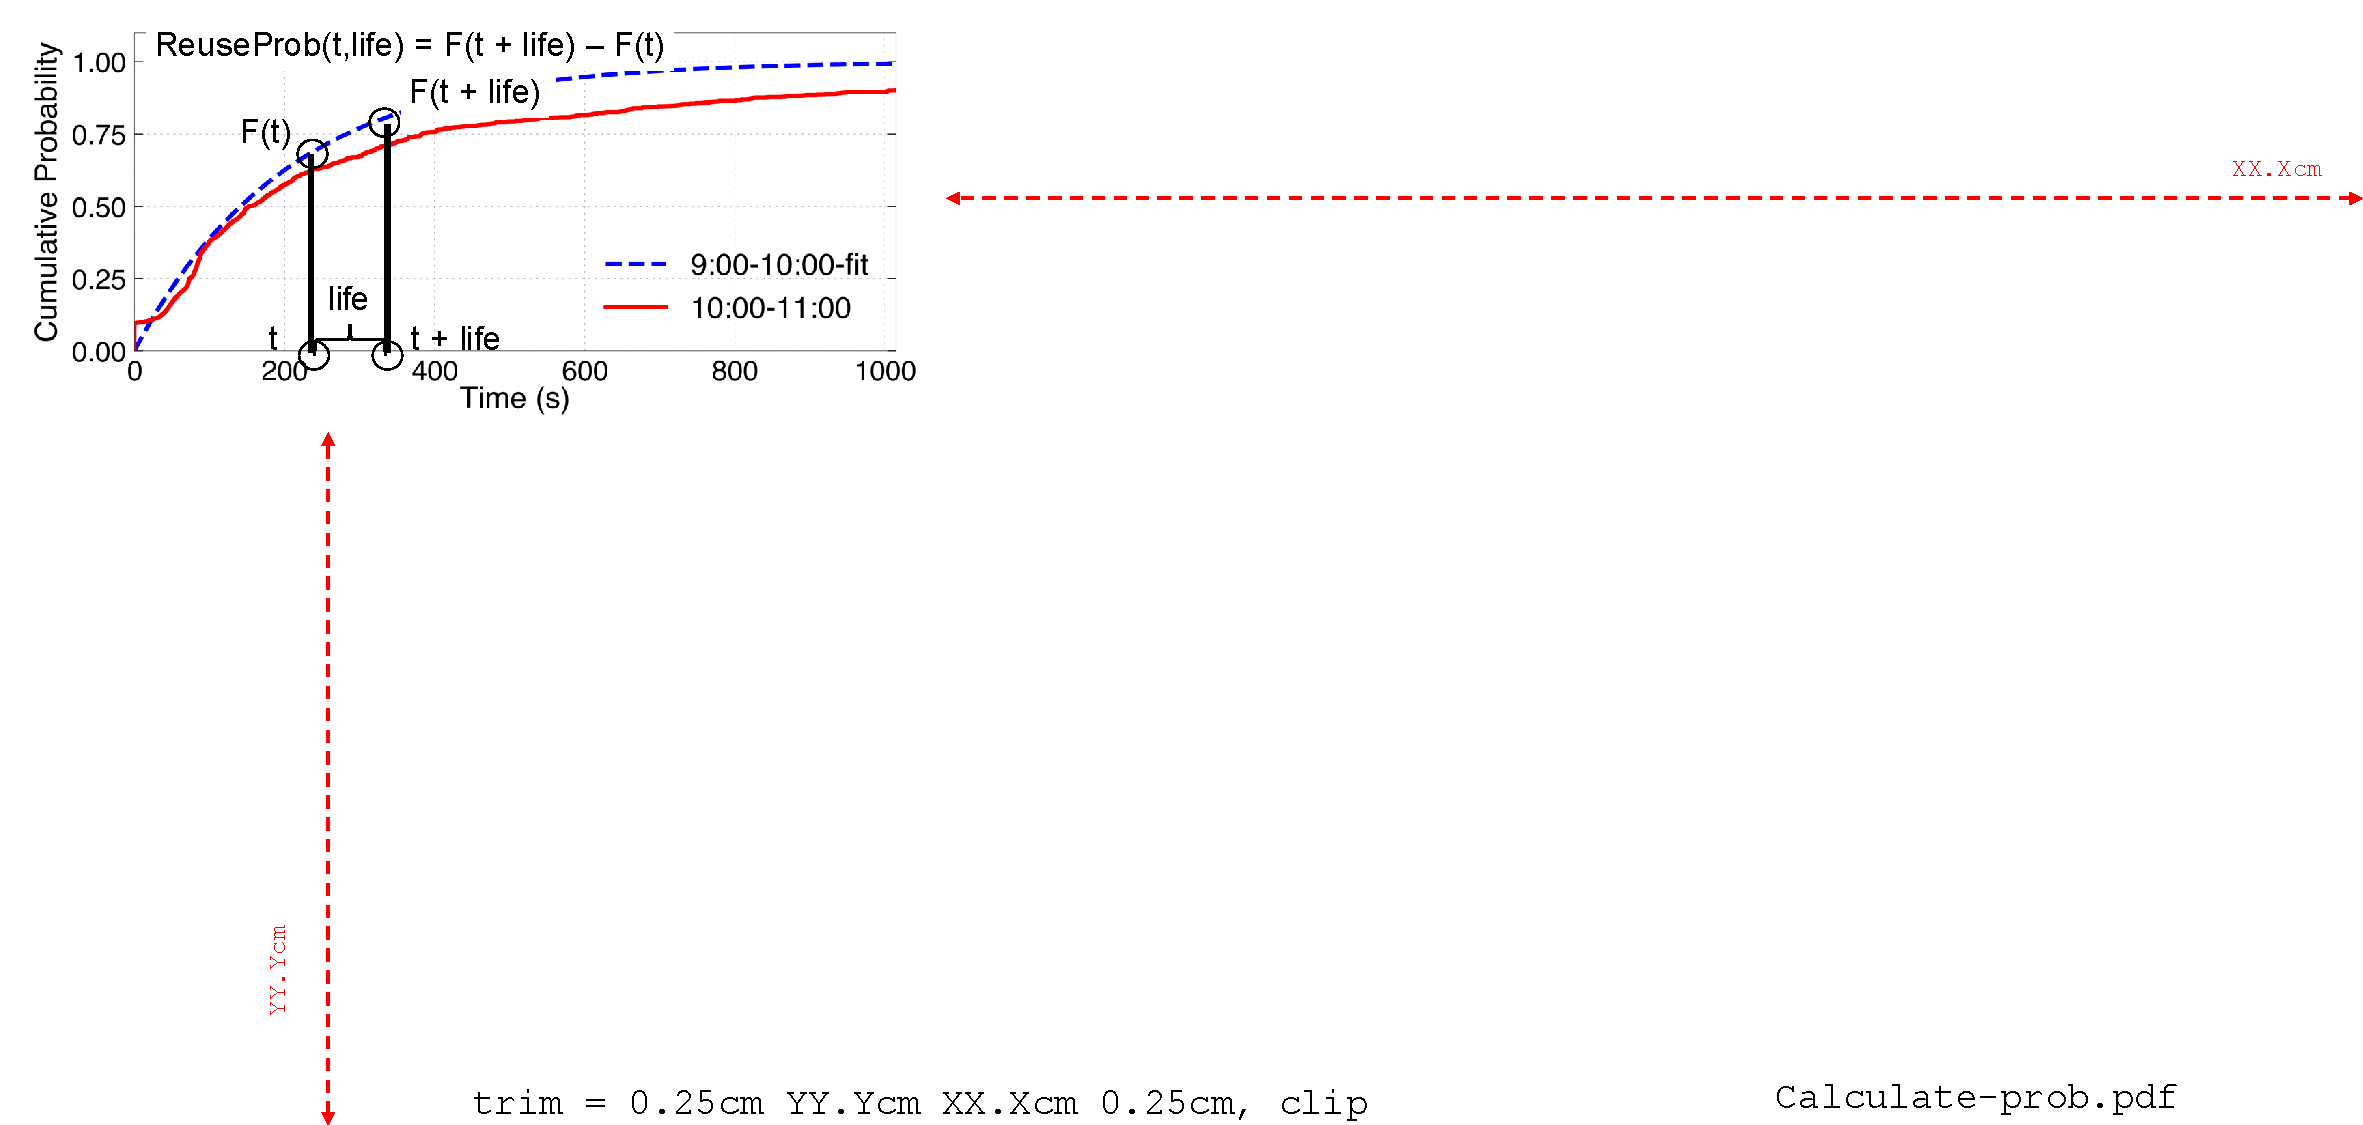
\includegraphics[width=.9\linewidth,trim=0.25cm 11.8cm 24cm 0.25cm,clip]{figs/calculate-prob.pdf}
    \caption{给定 {\kvcache} 块所属工作负载（请求类别）后，计算其复用概率的方法。}
    \label{fig:example-request-category}
\end{figure}

\stitle{本文策略。}
本文沿用 GDFS，为每个 {\kvcache} 块计算优先级并据此确定淘汰顺序，但用所刻画的 {\kvcache} 复用特征重新定义优先级：
\[
\text{Priority}=\bigl(\text{ReuseProb}_{w}(t,\text{life}),-\text{Offset}\bigr)
\quad(\text{工作负载感知}) .
\]
具体而言，优先级由包含两个指标的元组表示，并按字典序比较。两个指标背后的原理如下：
\begin{itemize}[leftmargin=*,itemsep=2pt]
    \item \textbf{ReuseProb$_w$}（\ding{192}）计算 {\kvcache} 块在给定时间 $t$ 的复用概率，其中 $t$ 表示距上次访问经过的时间。对每个工作负载（请求类别），复用概率按两步计算。第一，在后台采样最近一段时间内访问的数据。第二，依据\fig{fig:motiv-reuse-time-probability-hist}中的观察，用指数分布拟合采样数据，再查拟合曲线得到复用概率。\fig{fig:example-request-category}给出了计算示例：首先使用上午 9:00--10:00 的后台采样数据，拟合给定工作负载复用概率的累积分布函数（CDF，蓝线）。

    拟合曲线与真实数据（红线）十分接近。随后即可查曲线，得到一个 {\kvcache} 块未来的复用概率。该函数还考虑块的预期生命周期（life）；鉴于 {\kvcache} 生命周期很短，这一点至关重要。
    \item \textbf{Offset}（\ding{193}）考虑第~\ref{sec:motiv-temporal-spatial} 节描述的空间局部性：优先级与 {\kvcache} 块在整个请求中的前缀位置成反比。
\end{itemize}

本文不显式考虑频率（\ding{194}），因为即便对频繁复用的块而言，{\kvcache} 块的短暂生命周期（见\fig{fig:motiv-block-timespan}）也使频率无法为缓存策略提供有用信息。更重要的是，还必须用生命周期调节计算出的复用概率。否则，对于复用时间呈长尾分布的请求，拟合概率会在很长时间内返回较高值；这与 {\kvcache} 生命周期短暂的观察相矛盾，并会导致有限缓存空间利用低效。

\begin{figure}[!t]
    \centering
    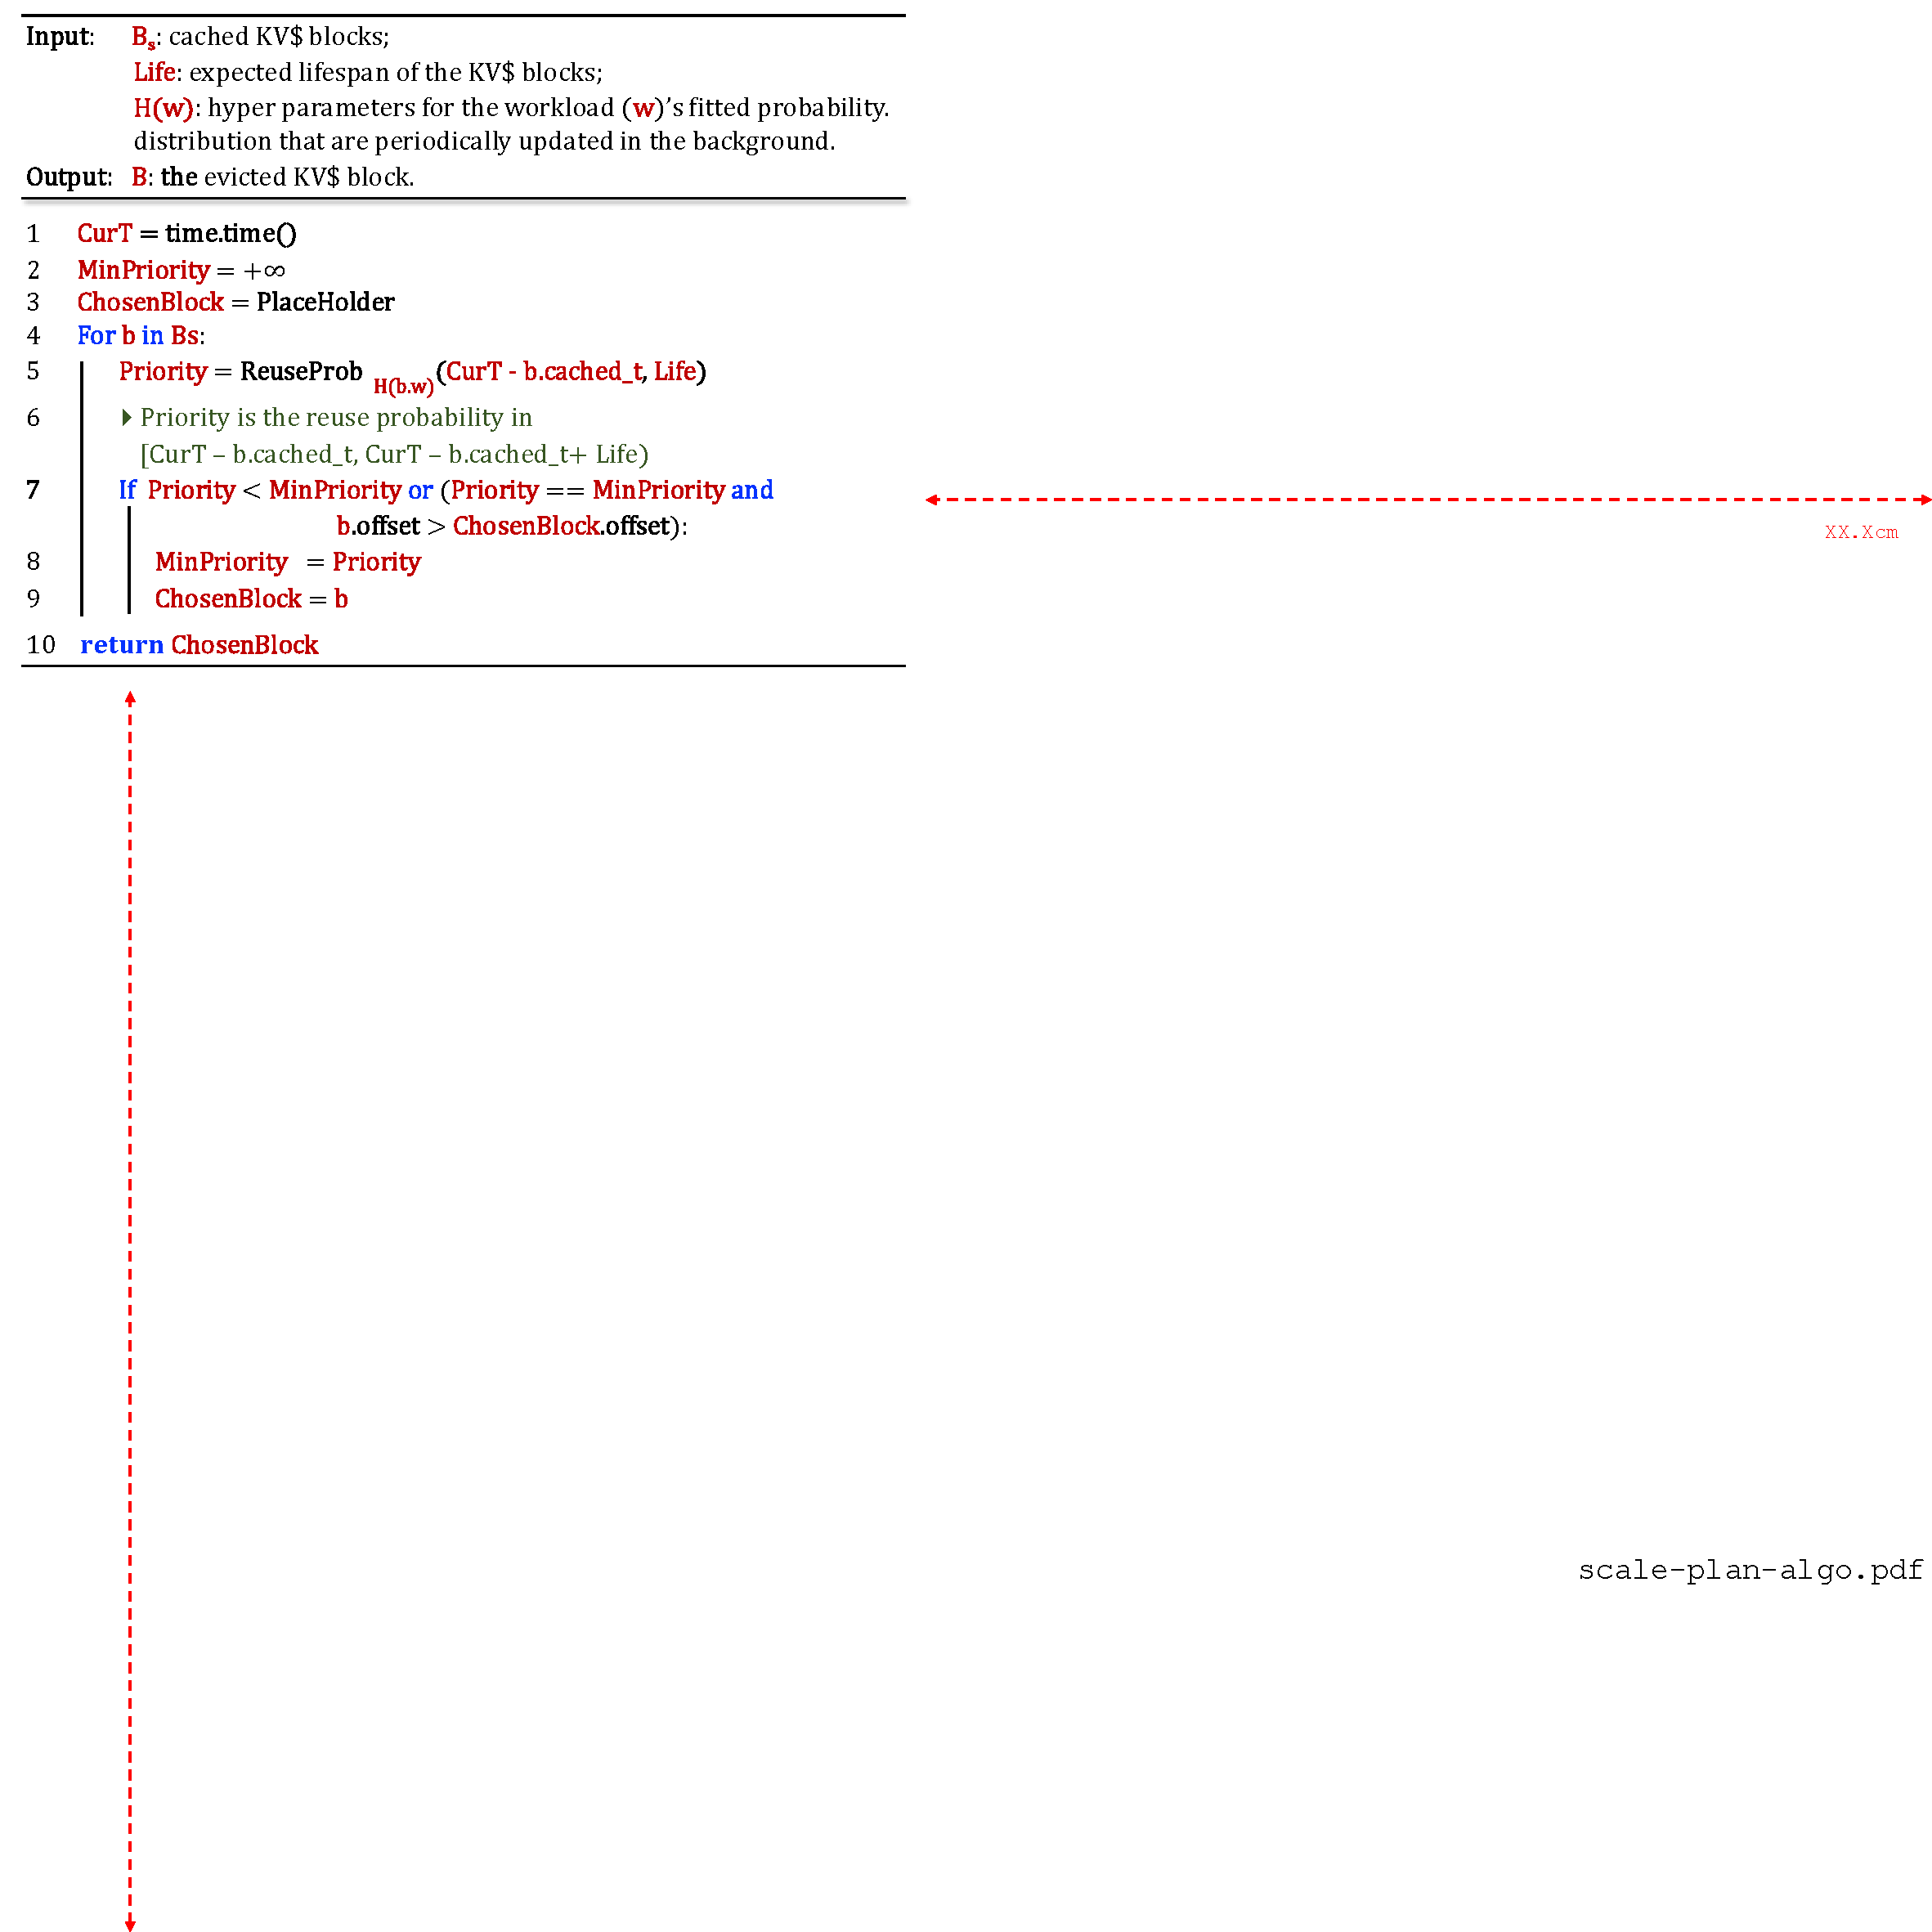
\includegraphics[width=\linewidth,trim=0.25cm 25.8cm 21cm 0.25cm,clip]{figs/naive-eviction-algo.pdf}
    \caption{本文工作负载感知缓存淘汰算法的简化伪代码。}
    \label{alg:naive-eviction}
\end{figure}

\stitle{详细淘汰算法。}
图~\ref{alg:naive-eviction}给出了工作负载感知缓存淘汰算法的简化伪代码。发生淘汰时，首先遍历所有缓存块（第 4--6 行），并使用块所属工作负载（$b.w$）计算每个块的复用概率；随后将优先级与块的偏移量一起比较，以更新待淘汰块（第 7--9 行）。

\stitle{性能优化。}
上述朴素算法的一个缺点是，必须计算所有 {\kvcache} 块的复用概率，才能找到最不可能复用的候选块。为避免过高计算开销，我们观察到：按照指数分布，每个工作负载内部的所有 {\kvcache} 块天然可按最后访问时间排序，因此比较同一工作负载中的块时无需计算复用概率。具体而言，对每个工作负载，维护一个按最后访问时间排序的 {\kvcache} 块优先队列。发生淘汰时，不再扫描所有块，而是先把每个工作负载中最近最少使用的块作为淘汰候选，然后运行图~\ref{alg:naive-eviction}所述算法得到最终淘汰块。这将复杂度从 $O(N)$ 降至 $O(W)$，其中 $W$ 是工作负载数量（通常为数十个）。因此，工作负载感知策略的服务性能开销可以忽略：本文观察到每次淘汰的策略延迟为 79\,$\mu$s，累计开销仅占典型服务引擎 vLLM~\cite{vllm} 调度开销的 1.2\,\%。

\subsection{性能评估}
\label{sec:design-eval}

\nospacestitle{测试平台。}
评估在一台配有 8 块 NVIDIA A800-80GB GPU 的服务器上进行。GPU 通过 400\,GBps 双向 NVLink 互连，因此可以使用多块 GPU（例如 4 块）通过张量并行~\cite{narayanan2021efficient}服务一个大模型。GPU 通过 PCIe Gen4 与主机连接，GPU HBM 与主机内存之间的双向带宽最高为 32\,GBps。

\stitle{实现与基线。}
由于 CachedAttention~\cite{cachedattention}和 Pensieve~\cite{DBLP:journals/corr/abs-2403-14401}等同时使用 CPU 与 GPU {\kvcache} 的先进缓存系统并未开源，本文在默认使用 GPU {\kvcache} 缓存的先进 LLM 服务系统 vLLM~\cite{vllm} 上实现了 CPU--GPU {\kvcache} 缓存，并进一步集成了先进系统中的策略与机制（见第~\ref{sec:design-mechanism} 节）。在相似测试平台和相同合成工作负载下，本文校准确认该实现的性能与 CachedAttention 等先进系统相近。

除在 vLLM 中集成 CPU {\kvcache} 缓存外，本文还实现了 Mooncake~\cite{mooncake}中的 {\kvcache} 中心化全局调度器，因为跨多个实例服务 LLM 十分常见。具体而言，全局调度器记录全局 {\kvcache} 缓存使用情况，并尽可能把请求调度到已经缓存相应 {\kvcache} 的实例。需要注意，本文工作负载感知缓存策略仅应用于单个服务实例；将其扩展到全局层留作未来工作。

\stitle{评估模型与工作负载。}
性能评估使用三个代表性开放模型：Qwen2-7B~\cite{qwen}、Llama2-13B~\cite{llama2}和 Llama3-70B~\cite{DBLP:journals/corr/abs-2407-21783}。选择这些模型的原因及其差异已在第~\ref{sec:analyze-capacity} 节的单请求 {\kvcache} 大小分析中讨论。Qwen2-7B 与 Llama2-13B 每个服务实例使用一块 GPU，Llama3-70B 使用四块 GPU。评估工作负载采用第~\ref{sec:workload-data} 节描述的轨迹 A 和 B。由于 GPU 数量不足以支持真实工作负载，本文使用保持轨迹时间模式的缩放方法~\cite{DBLP:conf/eurosys/SajalHZU021}，将轨迹缩放到测试平台的处理能力范围内。

\stitle{匿名轨迹上的评估方法。}
虽然轨迹已经匿名化，仍可通过构造精确复现原轨迹缓存命中模式的输入来评估系统服务性能。具体而言，对每个尚未分配 token 的匿名块，随机生成一个 token 列表，并确保每个生成列表的哈希都不同于其他列表。为匹配原始输入的迭代次数，还使用轨迹中的输出长度约束模型。最后，用构造的 token 替换模型生成输出，以保持多轮请求的缓存模式。

\begin{figure}[!t]
    \centering
    \includegraphics[width=\linewidth]{./data/qwen7b-cpu-cache-v2\figsuffix}
    \caption{Qwen2-7B 上缓存命中率、排队首 token 时间（QTTFT）与所配置 CPU 缓存之间的关系。}
    \label{fig:eval-qwen7b-cpu-cache}
\end{figure}

\begin{figure}[!t]
    \centering
    \includegraphics[width=\linewidth]{./data/llama13b-cpu-cache-v2\figsuffix}
    \caption{Llama2-13B 上缓存命中率、QTTFT 与所配置 CPU 缓存之间的关系。}
    \label{fig:eval-llama13b-cpu-cache}
\end{figure}

\begin{figure}[!t]
    \centering
    \includegraphics[width=\linewidth]{./data/llama70b-cpu-cache-v2\figsuffix}
    \caption{Llama3-70B 上缓存命中率、QTTFT 与所配置 CPU 缓存之间的关系。}
    \label{fig:eval-llama70b-cpu-cache}
\end{figure}

\stitle{缓存命中率提升。}
\fig{fig:eval-qwen7b-cpu-cache}--\ref{fig:eval-llama70b-cpu-cache}展示了标准缓存策略与本文工作负载感知策略（WA）的命中率和服务性能。比较基线包括最近最少使用（LRU）、先进先出（FIFO）、最不经常使用（LFU）以及近期优化的 FIFO 方法 S3-FIFO~\cite{10.1145/3600006.3613147}；原始 GDFS 则在\fig{fig:cache-policy-abl}中比较。

由于性能取决于缓存容量，本文通过改变所配置的 {\kvcache} 缓存容量来报告命中率与性能。容量相对于用于 {\kvcache} 的 GPU HBM 大小归一化，即图中的“\#CPU Cache / HBM”表示用于存储 {\kvcache} 的 CPU 内存相对于 GPU HBM 的比例。例如，该值为 1 表示用于存储 {\kvcache} 的 CPU 内存大小与 GPU HBM 相等。结果带来三项观察。

第一，与其他基线相比，本文策略 {\policy} 的命中率高 8.1--23.9\,\%；与其他基线中的最佳者相比，高 1.5--3.9\,\%。得益于对工作负载复用模式的了解，本文策略更有效。第二，缓存容量增大时，{\policy} 的有效性会降低；这符合预期，因为更大缓存能够容忍较低效的策略。最后，WA 在轨迹 A 上比在轨迹 B 上更有效，原因有二：（1）轨迹 B 几乎没有工作负载类别信息（$>99\,\%$ 的请求都是 1 轮请求），因此本文基于指数分布拟合的策略实质上退化为普通 LRU；（2）轨迹 B 所需的 {\kvcache} 容量较小，因此除 LFU 外，GPU HBM 已经接近最优。LFU 命中率较低，是因为最频繁访问的块也可能很早“死亡”，从而污染 {\kvcache} 缓存；前文已对此作了详细讨论。

\stitle{性能提升。}
缓存命中率提升会显著改善服务性能。\fig{fig:eval-qwen7b-cpu-cache}--\ref{fig:eval-llama70b-cpu-cache}还报告了服务不同轨迹时的排队 TTFT（QTTFT），即 TTFT 加上等待 GPU 处理请求的时间。得益于 {\kvcache} 命中率提高，{\policy} 将 QTTFT 降低了 28.3--41.9\,\%。

\begin{figure}[!t]
    \centering
    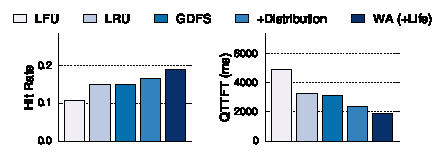
\includegraphics[width=\linewidth]{./data/abl.pdf}
    \caption{Qwen2-7B 上的消融研究，其中 \#CPU Cache / HBM 为 1。}
    \label{fig:cache-policy-abl}
\end{figure}

\stitle{消融研究。}
\fig{fig:cache-policy-abl}在轨迹 A 的 Qwen2-7B 模型上对不同策略进行消融研究；其他模型呈现相似趋势。首先，基于分布的方法使命中率提高 1\,\%（即表~\ref{tab:insights}中的技术\ding{192}）。使用生命周期调节器考虑 {\kvcache} 的短暂生命周期，又将命中率提高 2.4\,\%（\ding{194}）。需要注意，本文未单独描述局部性优化\ding{193}，因为它应用于所有策略。

\stitle{讨论：公平性问题。}
与所有现有系统及其策略一样，恶意客户端可以发送大量具有相同长前缀的请求来独占前缀缓存，从而造成公平性问题。保证公平性是与缓存策略彼此正交的议题，可以通过与 FairRide~\cite{DBLP:conf/nsdi/PuLZGS16,DBLP:conf/osdi/0007CLZ0ZGS24} 等 LLM 服务策略协同设计来解决。
